\section{Respuestas a las tres preguntas}

Las tres herramientas producen resultados idénticos, ya validados celda a celda, así que las respuestas se calculan una sola vez sobre la \textbf{versión XL: 38,215,560 viajes}, la más grande disponible.

\subsection{Q1: Demanda por hora del día y día de la semana}

\textbf{El patrón es bimodal en días laborables y unimodal en fin de semana.} La forma de las dos curvas es distinta, y esa diferencia es la respuesta.

De lunes a viernes aparecen dos picos de desplazamiento al trabajo: \textbf{08:00 h} con un promedio de 710,450 viajes y \textbf{17:00-18:00 h} con 660,092 y 606,309. Sábado y domingo tienen un único máximo aplanado a las \textbf{14:00 h}, con 439,431 viajes promedio: uso recreativo, no de transporte.

\begin{table}[htbp]
\centering
\caption{Hora pico y total por día de la semana}
\label{tab:q1-picos}
\begin{tabular}{lrrr}
\toprule
Día & Hora pico & Viajes en la hora pico & Total del día \\
\midrule
Lunes     & 17:00 & 672,240 & 5,590,150 \\
Martes    & 08:00 & 768,730 & 5,902,367 \\
Miércoles & 08:00 & 741,295 & 5,795,257 \\
Jueves    & 08:00 & 742,080 & 5,795,656 \\
Viernes   & 08:00 & 645,178 & 5,633,146 \\
Sábado    & 14:00 & 442,283 & 4,914,592 \\
Domingo   & 14:00 & 436,579 & 4,584,392 \\
\bottomrule
\end{tabular}
\end{table}

El pico laborable es 1.62 veces el pico de fin de semana. El valle nocturno está a las 03:00 h con 8,638 viajes promedio, y la franja de 00:00 a 05:00 h concentra apenas el \textbf{2.0\% del uso semanal}.

\textbf{Uso operativo:} las horas pico marcan cuándo la flota debe estar completa. La franja nocturna, con un 2\% del tráfico, es la ventana natural para mantenimiento y rebalanceo sin afectar el servicio.

Una advertencia de interpretación: el rango de fechas depende de la versión. Las versiones chicas cubren pocas semanas y pueden caer en período navideño, donde el patrón laborable aparece atenuado porque varios días hábiles son feriados. Comparar el mapa de calor entre versiones es en sí mismo un resultado, porque muestra que con pocos datos se puede llegar a una conclusión equivocada sobre estacionalidad.

\begin{figure}[htbp]
  \centering
  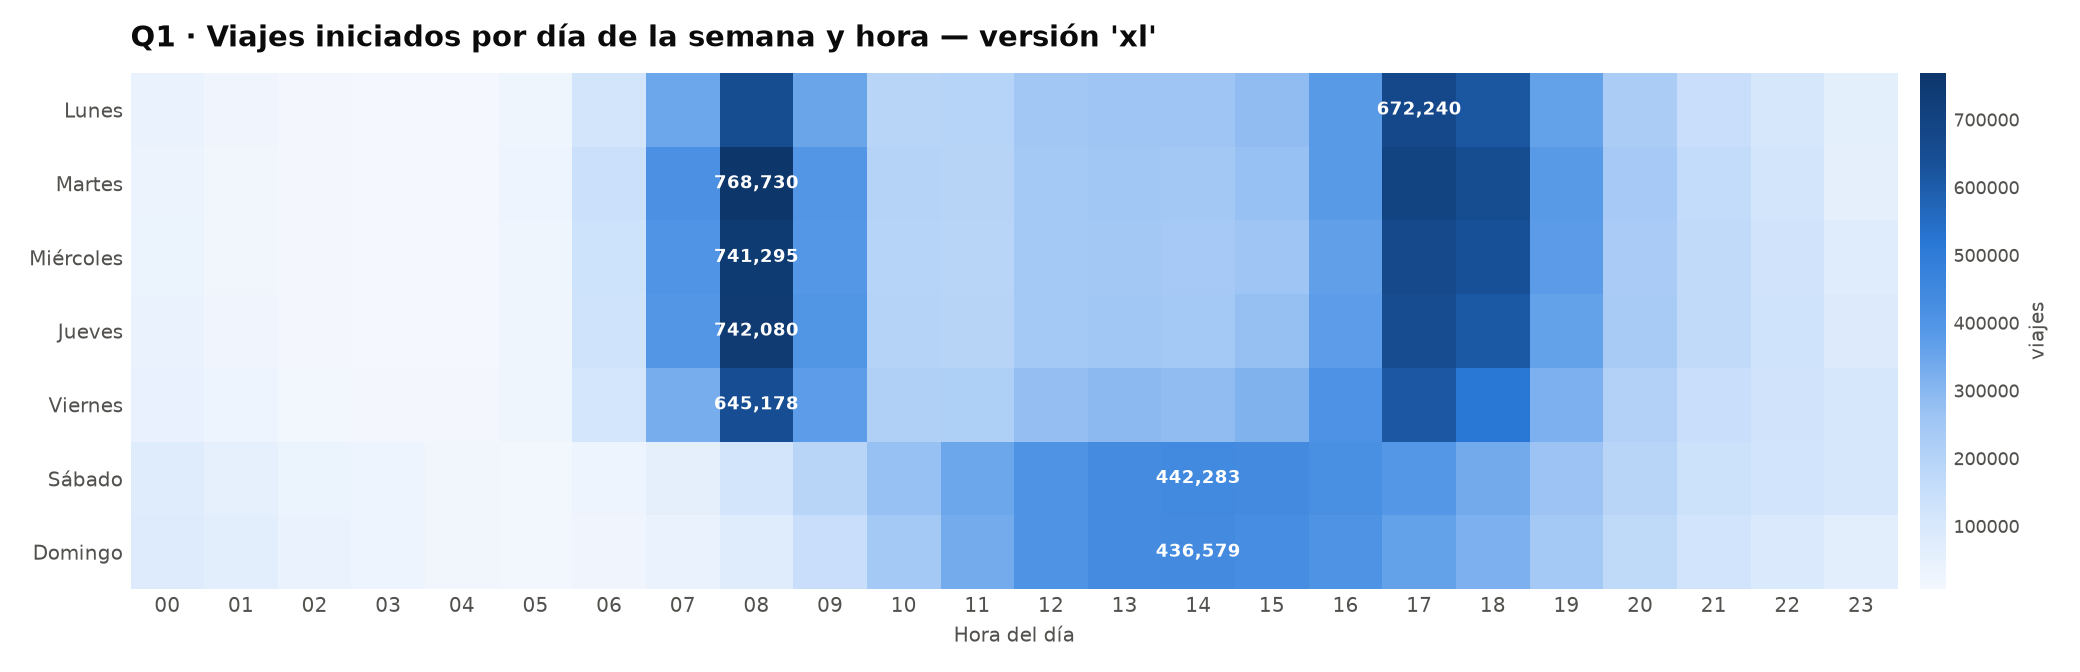
\includegraphics[width=0.8\textwidth]{figuras/q1_heatmap_xl.png}
  \caption{Mapa de calor de viajes por día de la semana y hora, versión XL.}
  \label{fig:q1-heatmap}
\end{figure}

\begin{figure}[htbp]
  \centering
  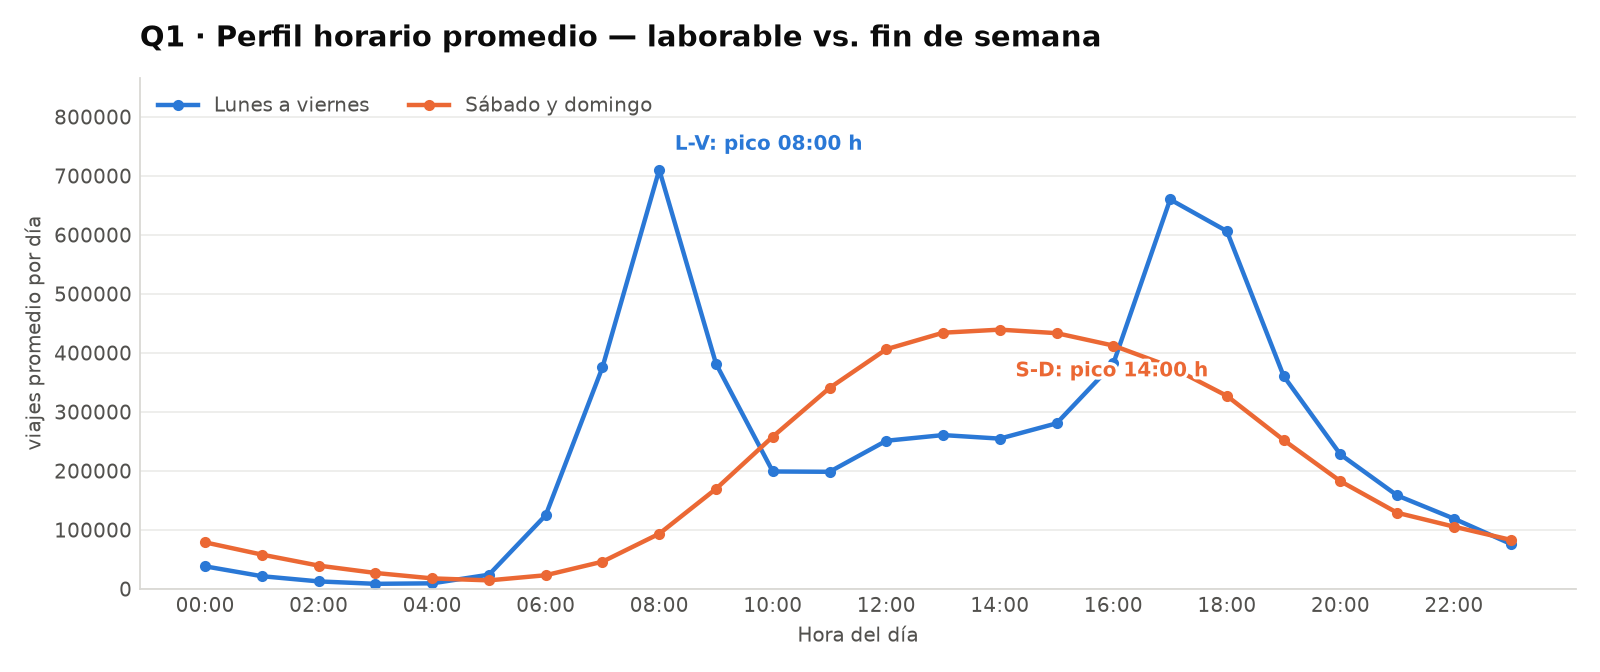
\includegraphics[width=0.8\textwidth]{figuras/q1_perfil_horario_xl.png}
  \caption{Perfil horario: días laborables vs. fin de semana, versión XL.}
  \label{fig:q1-perfil}
\end{figure}

\FloatBarrier

\subsection{Q2: Estaciones con mayor desequilibrio}

\textbf{El desbalance sigue el patrón radial clásico: déficit en nodos de transporte y periferia residencial, superávit en el núcleo financiero y comercial.} Con neto $=$ llegadas $-$ salidas, un valor negativo significa que la estación se vacía y hay que abastecerla; uno positivo, que se satura y hay que retirar bicicletas.

\begin{table}[htbp]
\centering
\footnotesize
\caption{Las cinco estaciones que más se vacían}
\label{tab:q2-deficit}
\begin{tabular}{lrrrr}
\toprule
Estación & Salidas & Llegadas & Neto & Desequilibrio \\
\midrule
Waterloo Station 2, Waterloo & 125,584 & 87,133 & $-38,451$ & $-18.1\%$ \\
Eagle Wharf Road, Hoxton & 107,628 & 86,866 & $-20,762$ & $-10.7\%$ \\
Cloudesley Road, Angel & 43,919 & 26,874 & $-17,045$ & $-24.1\%$ \\
Knightsbridge, Hyde Park & 51,202 & 37,693 & $-13,509$ & $-15.2\%$ \\
Notting Hill Gate Station, Notting Hill & 89,800 & 77,283 & $-12,517$ & $-7.5\%$ \\
\bottomrule
\end{tabular}
\end{table}

\begin{table}[htbp]
\centering
\footnotesize
\caption{Las cinco estaciones que más se saturan}
\label{tab:q2-superavit}
\begin{tabular}{lrrrr}
\toprule
Estación & Salidas & Llegadas & Neto & Desequilibrio \\
\midrule
Hop Exchange, The Borough & 176,231 & 237,045 & $+60,814$ & $+14.7\%$ \\
Holborn Circus, Holborn & 117,818 & 174,057 & $+56,239$ & $+19.3\%$ \\
St. James's Square, St. James's & 99,768 & 131,601 & $+31,833$ & $+13.8\%$ \\
Brushfield Street, Liverpool Street & 147,822 & 178,519 & $+30,697$ & $+9.4\%$ \\
Soho Square, Soho & 123,236 & 146,180 & $+22,944$ & $+8.5\%$ \\
\bottomrule
\end{tabular}
\end{table}

Waterloo Station encabeza el déficit, lo que confirma el patrón: la gente llega en tren y toma una bicicleta hacia el centro por la mañana. Holborn, Borough y St. James's son distritos de oficinas, y ahí es donde esas bicicletas terminan.

\textbf{Magnitud absoluta contra magnitud relativa.} El neto ordena por volumen, pero el porcentaje revela estaciones medianas con desbalance proporcional severo. Filtrando a estaciones con más de 20,000 viajes, los casos más críticos en términos relativos son \textbf{New North Road 1, Hoxton ($-26.9\%$)}, \textbf{Risinghill Street, Angel ($-25.2\%$)} y \textbf{Cloudesley Road, Angel ($-24.1\%$)}. El barrio de Angel aparece tres veces: es una zona residencial que se vacía sistemáticamente cada mañana. Para operaciones el porcentaje suele importar más que el absoluto, porque una estación que pierde una cuarta parte de su inventario está vacía buena parte del día.

\textbf{Sesgo declarado:} 68,213 viajes (0.18\% del total) no tienen estación de destino registrada. Cuentan como salida y no como llegada, así que empujan el neto hacia el déficit. El efecto es pequeño frente a las magnitudes reportadas, pero existe.

\begin{figure}[htbp]
  \centering
  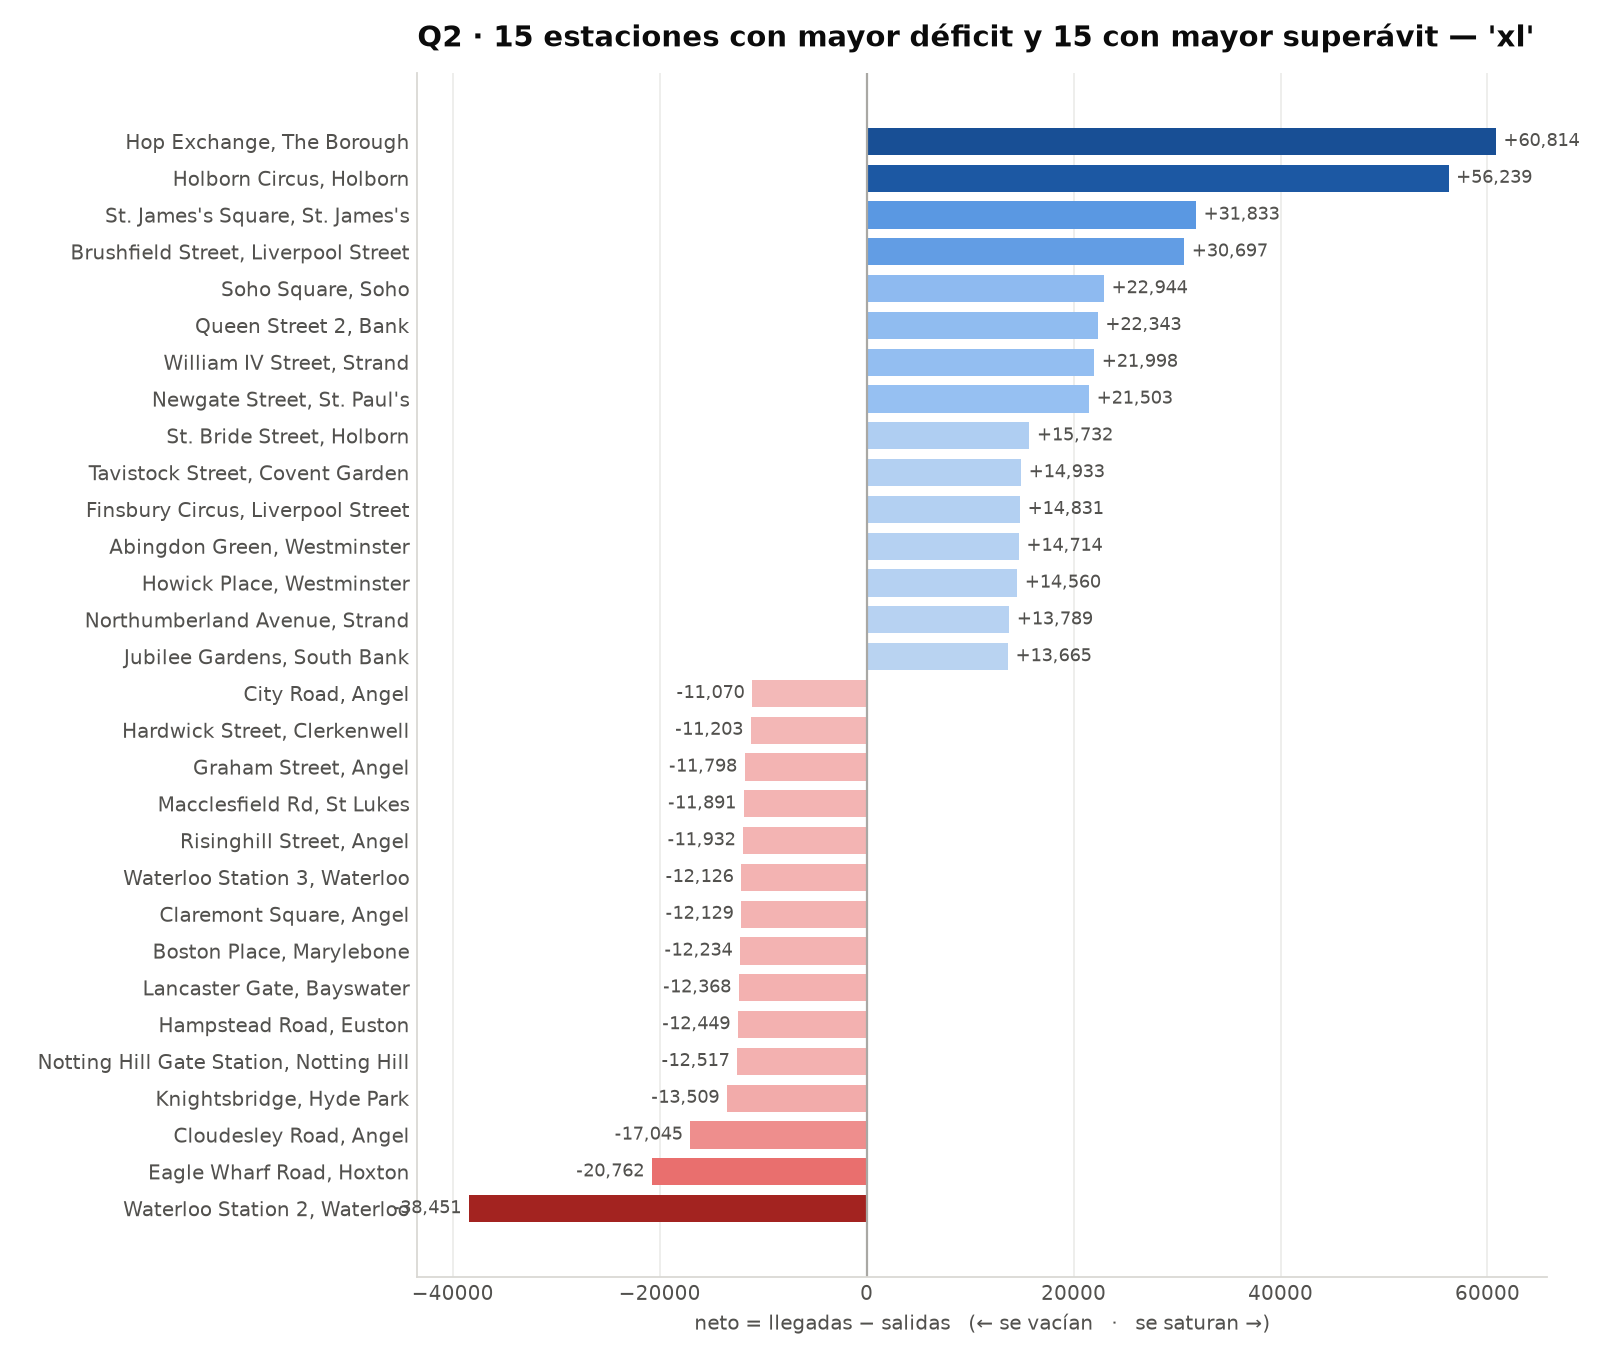
\includegraphics[width=0.8\textwidth]{figuras/q2_desequilibrio_xl.png}
  \caption{Estaciones con mayor déficit y superávit, versión XL.}
  \label{fig:q2-desequilibrio}
\end{figure}

\begin{figure}[htbp]
  \centering
  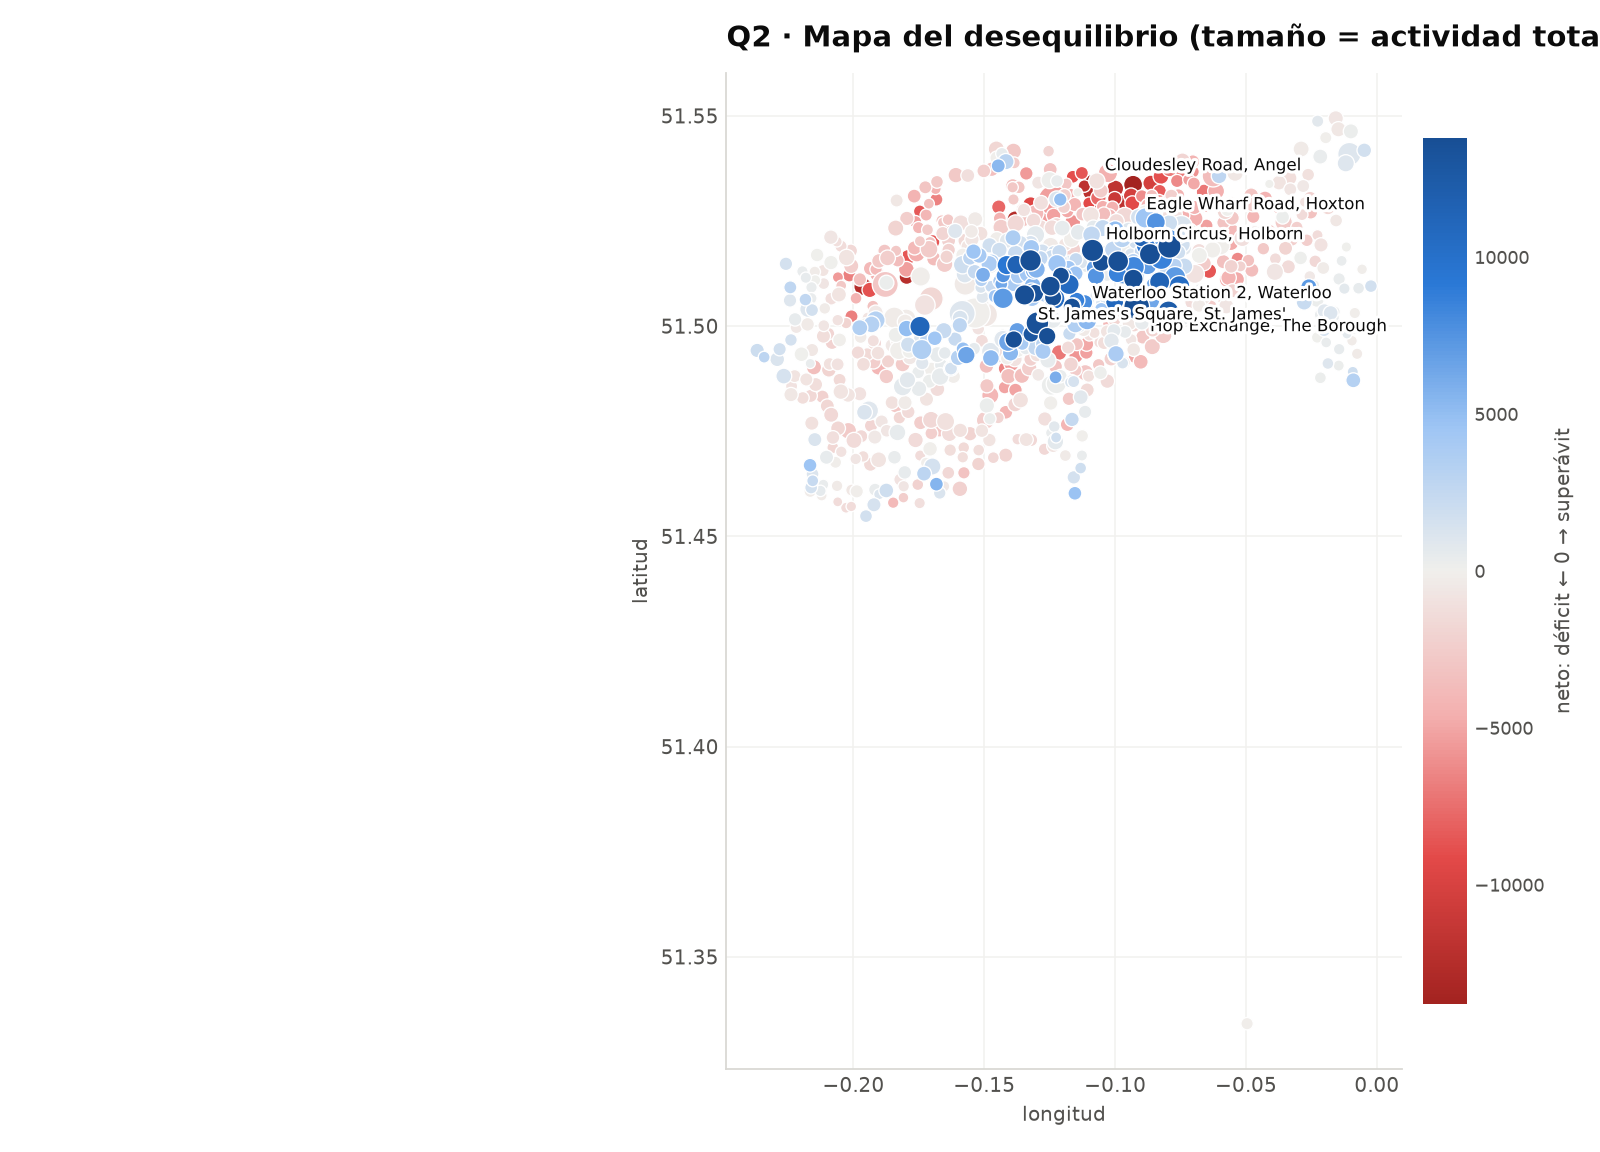
\includegraphics[width=0.8\textwidth]{figuras/q2_mapa_xl.png}
  \caption{Mapa geográfico del desbalance por estación, versión XL.}
  \label{fig:q2-mapa}
\end{figure}

\FloatBarrier

\subsection{Q3: Concentración del tráfico en rutas}

\textbf{Sí hay concentración, pero no es un Pareto 80/20: la forma es de cola extremadamente larga.} Sobre 652,864 pares origen-destino teóricamente posibles (808 estaciones al cuadrado), solo 510,672 aparecen alguna vez. Las \textbf{1,000 rutas más transitadas concentran el 9.6\% de todos los viajes}, y las 20 primeras apenas el 1.35\%.

\begin{table}[htbp]
\centering
\footnotesize
\caption{Rutas más transitadas, versión XL}
\label{tab:q3-rutas}
\begin{tabular}{clrr}
\toprule
\# & Ruta & Viajes & \% del total \\
\midrule
1  & Hyde Park Corner $\rightarrow$ Hyde Park Corner & 72,625 & 0.190\% \\
2  & Aquatic Centre $\rightarrow$ Aquatic Centre (Olympic Park) & 67,661 & 0.177\% \\
3  & Albert Gate $\rightarrow$ Albert Gate (Hyde Park) & 42,049 & 0.110\% \\
4  & Black Lion Gate $\rightarrow$ Black Lion Gate (Kensington Gardens) & 40,221 & 0.105\% \\
5  & Triangle Car Park $\rightarrow$ Triangle Car Park (Hyde Park) & 35,652 & 0.093\% \\
10 & Hyde Park Corner $\rightarrow$ Triangle Car Park & 15,739 & 0.041\% \\
11 & Hyde Park Corner $\rightarrow$ Albert Gate & 15,405 & 0.040\% \\
\bottomrule
\end{tabular}
\end{table}

Tres lecturas:

\begin{enumerate}
  \item \textbf{Las rutas circulares dominan el top y no son viajes de transporte.} Las nueve rutas más transitadas tienen origen igual a destino, y todas están en parques: Hyde Park, Kensington Gardens y el Queen Elizabeth Olympic Park. Son paseos recreativos, no desplazamientos. En las primeras 1,000 rutas hay 208 circulares que suman 1,026,226 viajes. Mezclarlas con los desplazamientos punto a punto distorsiona cualquier conclusión sobre movilidad, así que se marcan aparte.
  \item \textbf{Los corredores estructurales aparecen después.} Las rutas no circulares del top conectan puntos dentro de los mismos parques o nodos de transporte con distritos de oficinas. Son el último tramo del trayecto al trabajo y candidatas naturales a carril exclusivo o a más capacidad de anclajes.
  \item \textbf{La cola larga justifica la red.} Que ninguna ruta individual supere el 0.2\% del tráfico significa que el valor del sistema está en la cobertura, no en unos pocos corredores. Optimizar unas decenas de rutas tiene impacto local; mantener la red completa es lo que la hace útil como red.
\end{enumerate}

\textbf{Relación entre Q2 y Q3.} Una ruta asimétrica, con mucho tráfico A$\rightarrow$B y poco B$\rightarrow$A, es la \textbf{causa} del desequilibrio que Q2 mide como \textbf{efecto}. Cruzar ambas identifica qué corredor concreto genera cada estación deficitaria, que es la información que necesita el equipo de rebalanceo. Y cruzar Q2 con Q1 daría la ventana horaria en que conviene intervenir, porque una estación puede vaciarse por la mañana y llenarse por la tarde.

\begin{figure}[htbp]
  \centering
  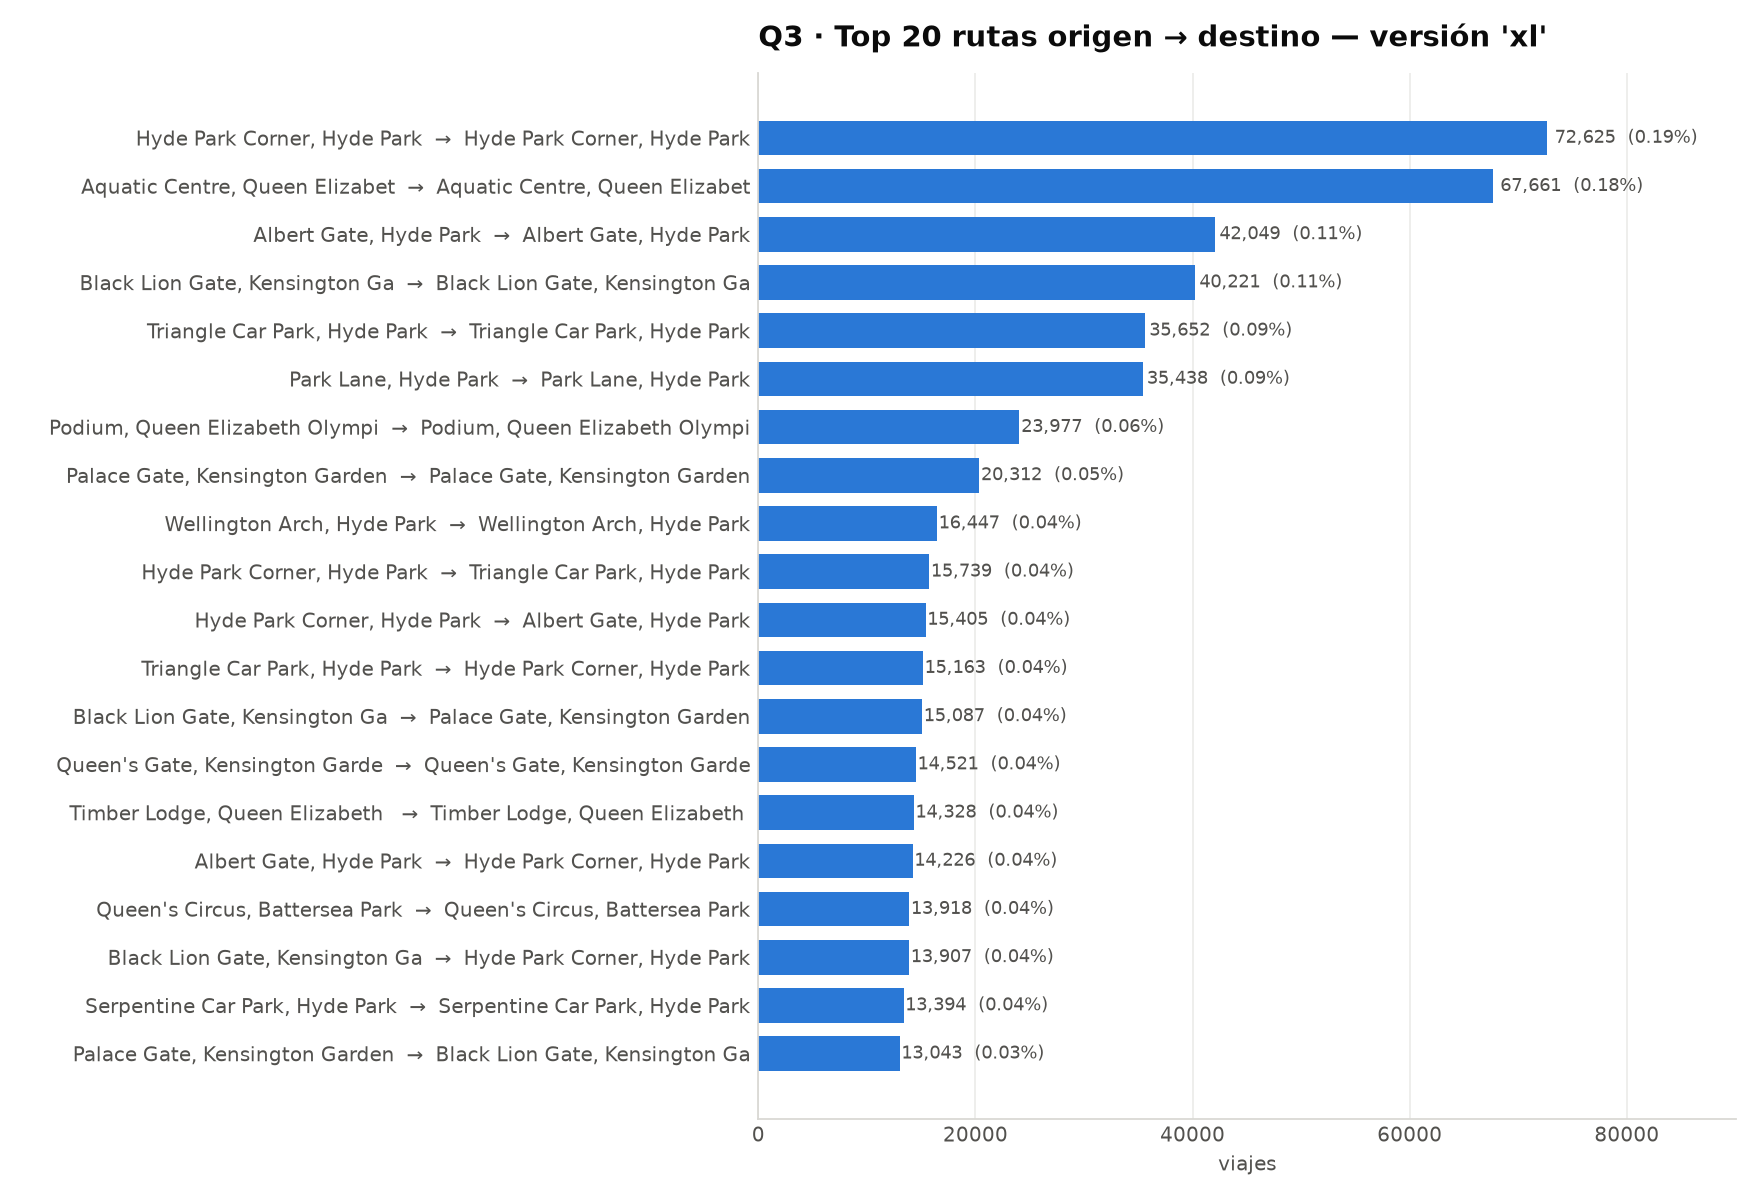
\includegraphics[width=0.8\textwidth]{figuras/q3_top_rutas_xl.png}
  \caption{Top 20 rutas más transitadas, versión XL.}
  \label{fig:q3-toprutas}
\end{figure}

\begin{figure}[htbp]
  \centering
  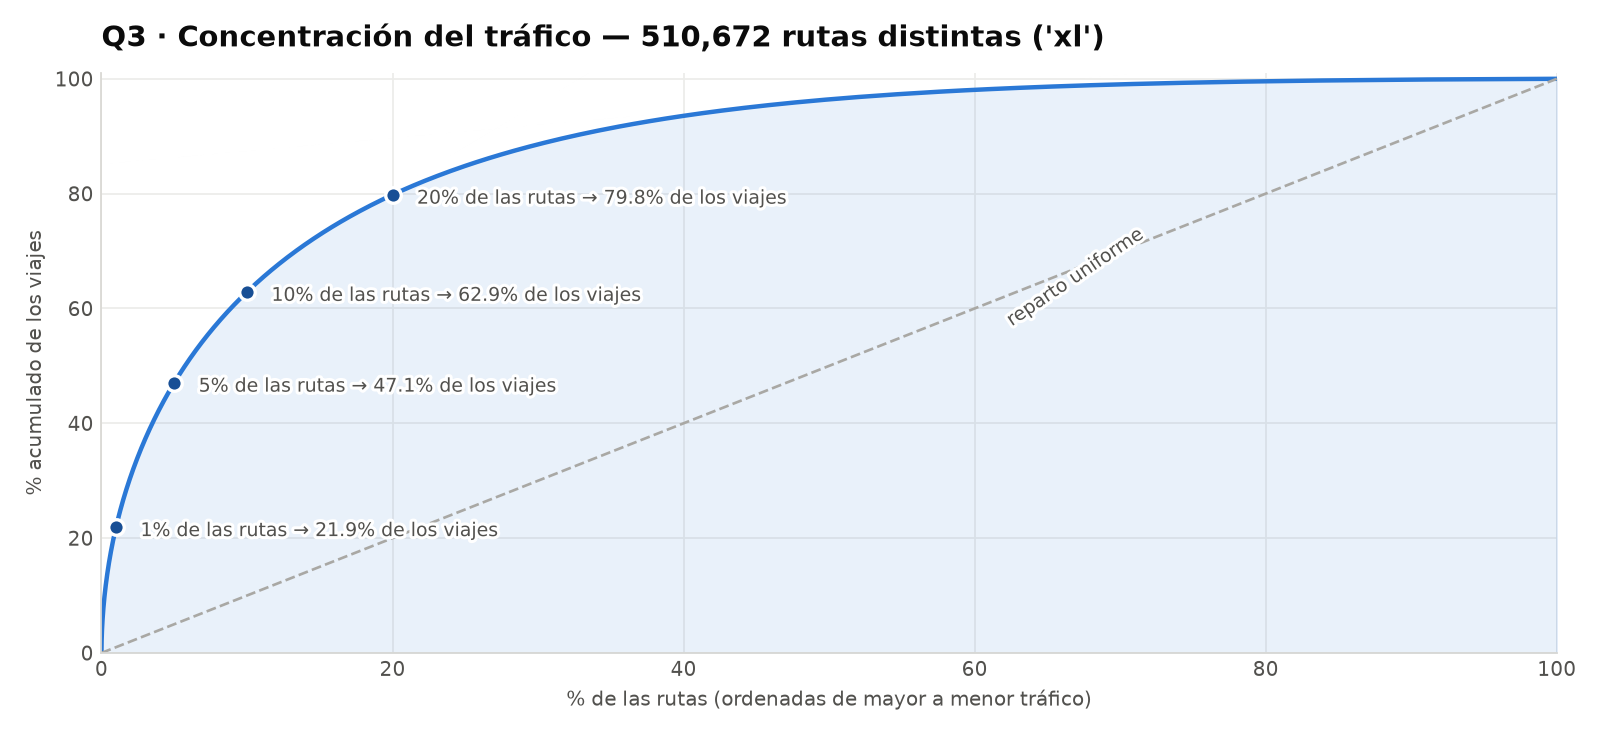
\includegraphics[width=0.8\textwidth]{figuras/q3_pareto_xl.png}
  \caption{Curva de concentración (Pareto) del tráfico por ruta, versión XL.}
  \label{fig:q3-pareto}
\end{figure}
